\chapter{Designing a Collaborative Modeling Framework}

In this chapter, the collaborative modeling framework will be explained in depth. The target platform for applications modeled through the framework is Android. Once a modeler has a basic understanding of how Android development works, the modeler can use this framework to rapidly develop Android collaborative prototype applications. In the first section, we will give an overview of all the formalisms and technologies used in the form of a Megamodel. Next, we will describe the basic building blocks of the framework through a class diagram and discuss the meta-models that make up the core of an Android application. In the third section we describe the server component, written in Node.js \cite{NodeJS} and Javascript. The server component is used to persist data created by a user and to distributed this data to other users currently involved in a session. Finally, we end the chapter with a section on code generation and EGL \cite{EGL}.

\section{Megamodel}

Modeling-in-the-large, or \textit{Megamodeling}, considers the global relationships between models, meta-models and all formalisms used in general, without considering their context \cite{Megamodeling}. In \cite{Megamodeling}, they describe the concept of Megamodeling as follows:
\begin{quotation}
For instance for a model to be useful, one needs a metamodel but also transformations that operates on it, and then transformation engines to interpret the transformation models, interpreters to interpret the language in which the transformation engines are written in, and so on. A megamodel is a model that represents this kind of complex arrangements without entering into the details of each artefact.
\end{quotation}
In this section, we will give an overview of all the artifacts used in the design and implementation of this work. This megamodel is depicted in figure ~\ref{fig:megamodel}.
\begin{figure}[h!]
\centering
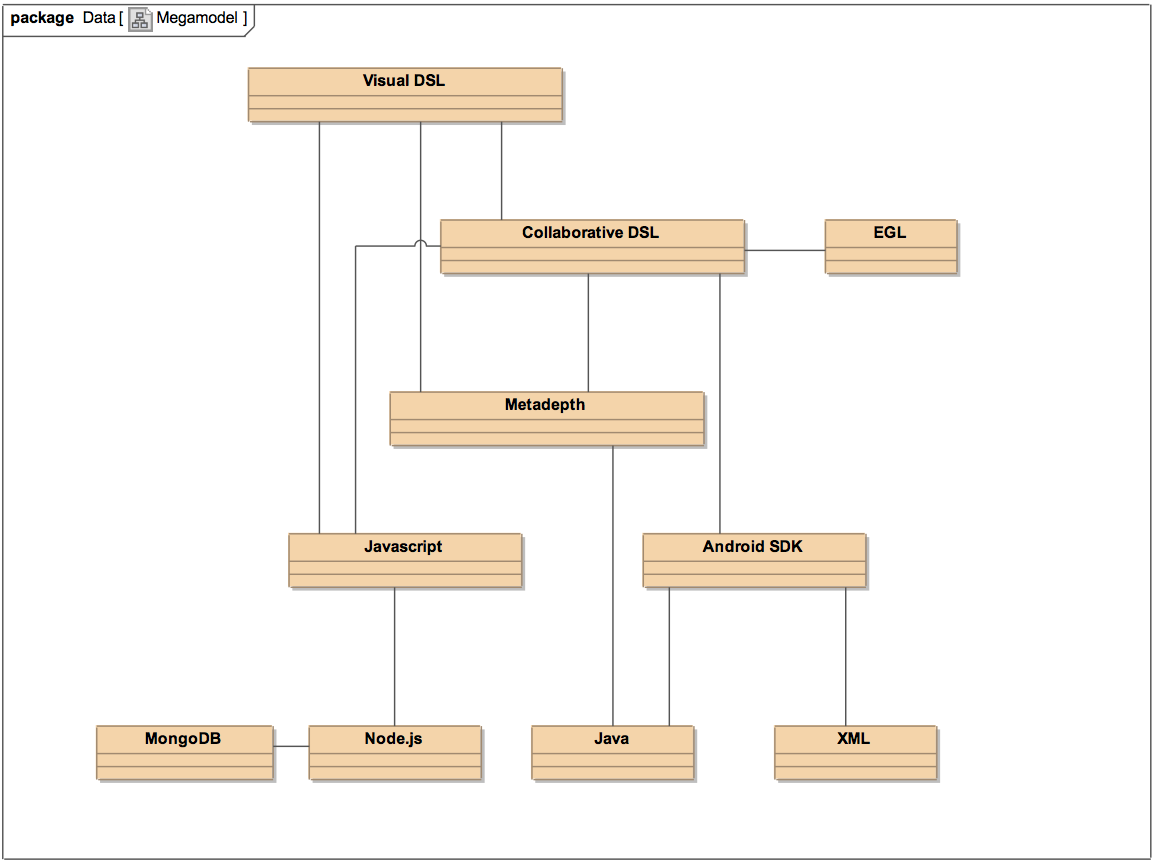
\includegraphics[width=1.02\textwidth]{images/chap6_megamodel.png}
\caption{Megamodel.}
\label{fig:megamodel}
\end{figure} \\
On the lowest levels we see all the technologies used in this work, such as Javascript, Java and XML.  On the highest level, we see the Visual DSL (see Appendix A) that uses both Javascript (to generate the visual environment itself), Metadepth (to define the meta-models) and the collaborative DSL (to provide a target mapping for a model transformation). The lines between the formalisms describe associations. For instance, the collaborative modeling framework (which is the DSL and all the build tools) uses the Android SDK, Metadepth and Javascript to build its DSL.

\section{Main component Meta-models}

In this section, we will discuss the main component meta-models featured in the collaborative modeling framework. First, a high-level overview in the form of a class diagram will be given. Next, individual meta-models will be explained in more detail.

\subsection{High-level class diagram}

In figure ~\ref{fig:highlevel_mm}, we see a high-level overview class diagram. This class diagram contains all the important meta-models that make up an application model in the framework. There is one important piece missing in the class diagram, which is the \texttt{Component} hierarchy. This hierarchy will be reviewed in section 6.3. The meta-models \texttt{Application}, \texttt{Manifest}, \texttt{Activity}, \texttt{AndroidAction}, \texttt{UIAction} and \texttt{Server} will be explained in detail in this chapter. 
\begin{figure}[h!]
\centering
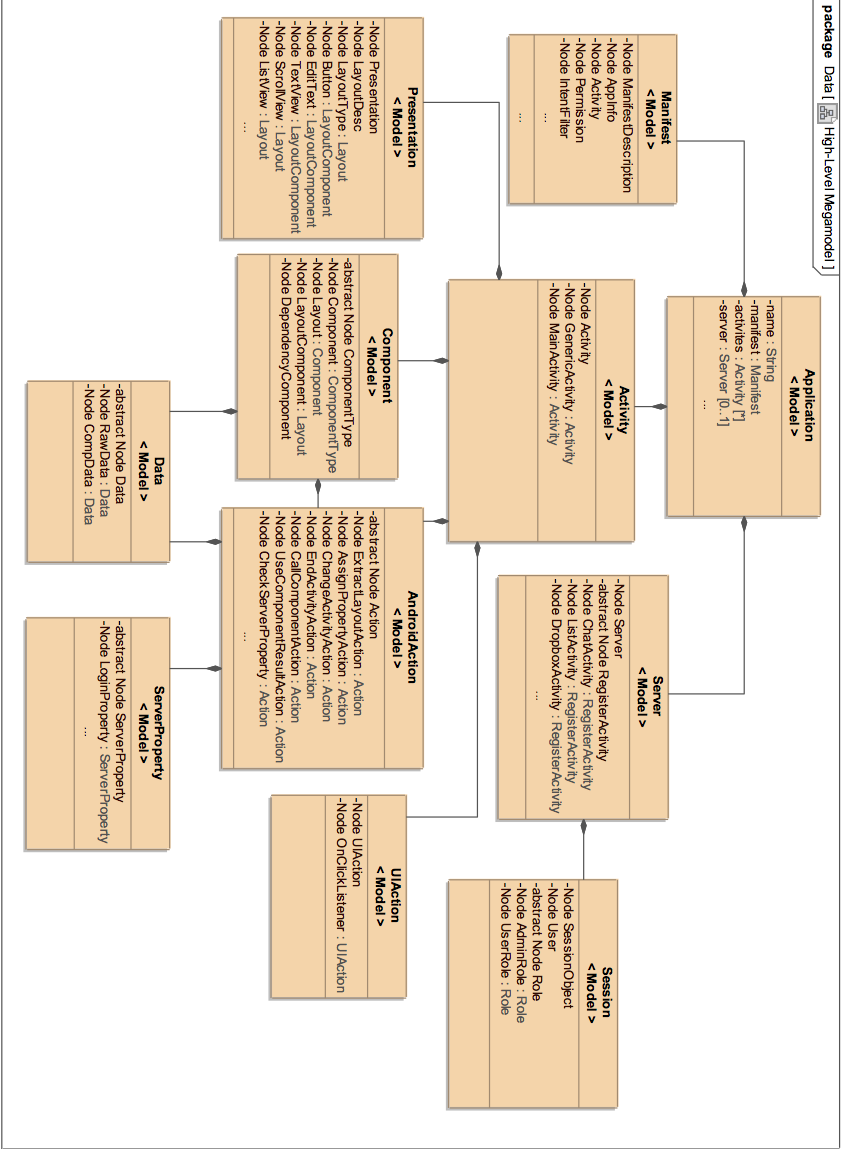
\includegraphics[width=1.02\textwidth]{images/chap6_high_level.png}
\caption{High-level Class Diagram.}
\label{fig:highlevel_mm}
\end{figure}

\subsection{Application}

The top-level meta-model that represents an Android application is the \texttt{Application} meta-model. \texttt{Application} has a \texttt{name} field and contains an \texttt{AndroidManifest} and a set of \texttt{Activities}. If we want to communicate with a server, we also need to specify an instance of the \texttt{Server} meta-model. The complete \texttt{Application} meta-model is described as follows:

\begin{lstlisting}[label=application-mm,caption=Application meta-model, captionpos=t]
load "Manifest"
load "Activity"
load "Server"

Model Application imports Activity, Manifest, Server {
	name			: String;
	manifest		: ManifestDescription[1];
	activities		: Activity[*];
	server 			: Server[0..1];
}
\end{lstlisting}

\subsection{Manifest}

One field in the \texttt{Application} meta-model is the \texttt{AndroidManifest}. The \textit{AndroidManifest.xml}, as described in chapter 4, contains all activities and other Android components. The equivalent meta-model is declared as follows:

\begin{lstlisting}[label=application-mm,caption=Manifest meta-model, captionpos=t]
Model Manifest {

	Node ManifestDescription {
		namespace		: String="http://schemas.android.com/apk/res/android";
		package			: String;
		versionCode		: String="1";
		versionName		: String="1.0";
		sdk				: String;
		app_info		: AppInfo[1];
		permissions		: Permission[*];
	}

	Node AppInfo {
		icon 		: String="@drawable/icon";
		label		: String="@string/app_name";

		activities	: Activity[*];
	}

	// e.g. <uses-permission android:name="android.permission.SEND_SMS"/>
	Node Permission {
		name 	: String;
	}

	Node Activity {
		name 	: String;
		label 	: String="@string/app_name";
		intent	: IntentFilter;
	}

	// e.g. http://developer.android.com/guide/topics/intents/intents-filters.html
	Node IntentFilter {
		action 		: String="android.intent.action.MAIN";
		category	: String="android.intent.category.LAUNCHER";
	}
}
\end{lstlisting}
Some of the fields have a pre-defined value, such as \texttt{namespace}, \texttt{icon} or \texttt{label}. Other fields need to be set explicitly by the modeler. The \texttt{package} field describes the Java package used to logically organize the source code. Other fields describe the current SDK version of Android and the Activities that correspond with the ones that are modeled in the \texttt{Activity} meta-model. The \texttt{Permission} Node models the permissions that the modeled application needs. For instance, if the application needs to access the internet, we need to add an INTERNET permission. Every Android application can have a variety of permissions set to use the functionality provided by the SDK \cite{AndroidPermissions}. An \texttt{IntentFilter} is associated to an Activity, we indicate that this Activity is the entry point of the application. In Android, other options can be specified through intent filters \cite{AndroidIntentFilter}, but these are not supported in the collaborative modeling framework.

\subsection{Activity}

The most important part of the collaborative framework is the \texttt{Activity} meta-model. It encapsulates all Android components, the layout and all actions on (layout) components. The \texttt{Activity} meta-model is designed as follows:

\begin{lstlisting}[label=activity-mm,caption=Activity meta-model, captionpos=t]
load "Presentation"
load "Component"
load "AndroidAction"
load "UIAction"

Model Activity imports Presentation, Component, AndroidAction, UIAction {

	Node Activity {
		name				: String;
		// Is this the main activity that is launched when launching the application?
		main 				: boolean;

		content				: Component@0[*];
		presentation		: Presentation[1];
		onClickListeners 	: UIAction[*];
	}

}
\end{lstlisting}
As we can see, an Activity contains an arbitrary number of components (explained in next section), a presentation model and a set of UI actions. Both the \texttt{Presentation} and \texttt{Action}/\texttt{UIAction} meta-models will be explained in next subsections.

\subsection{Presentation}

In this section, we will review the \texttt{Presentation} meta-model. This meta-model represents a mapping from the Metadepth syntax to the XML representation in Android. The \texttt{Presentation} meta-model is described in Listing ~\ref{presentation-mm}
%In an Android application, the layout of an Activity is usually presented through an XML file. Alternatively, the layout of an \texttt{Activity} can also be described through Java code. For the collaborative modeling framework, the XML approach was chosen, so the code generation part will generate a set of XML files that represent the application's layout.

\begin{lstlisting}[label=presentation-mm,caption=Presentation meta-model, captionpos=t]
load "Component"

Model Presentation imports Component {
	
	Node Presentation {
		activityname 	: String;
		layout 			: LayoutDesc[1];
	}

	Node LayoutDesc {
		name			: String;
		layoutType		: LayoutType[1];
	}

	// e.g. LinearLayout
	Node LayoutType : Layout {
		name 		: String;
		namespace	: String="http://schemas.android.com/apk/res/android";
		orientation	: String;
		width		: String="fill_parent";
		height		: String="fill_parent";

		children 	: Layout@0[*];
	}

	Node Button : LayoutComponent { }

	Node EditText : LayoutComponent {
		password 		: String;
		requestFocus	: boolean;
	}

	Node TextView : LayoutComponent { }

	Node ScrollView : Layout {
		width 		: String;
		height 		: String;
		weight 		: String;
		components 	: Layout@0[*];
	}

	Node ListView : Layout {
		width		: String;
		height		: String;
		weight		: String;
	}
}
\end{lstlisting}
The relevant part of the meta-model is defined through the \texttt{LayoutType} node. This node describes the type of layout (e.g. LinearLayout, a layout that arranges its children in a single row or column \cite{AndroidLinearLayout}) to use in the \texttt{Activity}. Apart from the type, it also contains a description of the elements contained in the layout itself. We usually want to create a \texttt{LinearLayout} type, but other types are possible too \cite{AndroidLayoutType}. Examples of layout elements are \texttt{Button} or a child view that has its own layout elements, for example a \texttt{ScrollView}.

\subsection{Action}

The \texttt{Action} meta-model is an important part in the functionality of the collaborative modeling framework. It provides a skeleton for executing actions on Android components or elements in a layout. Another example of an action would be the exchange of data between activities. A part of the \texttt{Action} meta-model is displayed in listing ~\ref{androidaction-mm}.

\begin{lstlisting}[label=androidaction-mm,caption=AndroidAction meta-model, captionpos=t]
load "Component"
load "ServerProperty"
load "Data"

Model AndroidAction imports Component, ServerProperty, Data {
	
	abstract Node Action {
		ctype			: String{id};
		condition 		: Action;
	}

	// e.g. use the value of a text field to call the action method of a component
	Node ExtractLayoutAction : Action {
		source 			: Component@0;
		name 			: String;
	}

	// Specify the target activity
	Node ChangeActivityAction : Action {
		oldActivity 	: String;
		newActivity 	: String;
		data 			: Data[*];
	}

	// Call the action method of a component.
	// Might save a value if it's a sensor (i.e. geo)
	// Or execute a real action if it's an actuator (i.e. send an SMS)
	Node CallComponentAction : Action {
		// properties needed to call the action method of the component
		properties		: Data[*];
	}
}
\end{lstlisting}
The actions listed above are the three most used and important actions. The \texttt{ExtractLayoutAction} takes as arguments a source layout component and a name for the data that has to be extracted. This data will be extracted from the source component that is specified. Usually this is an Android \texttt{TextView} or \texttt{EditText} component. The \texttt{ChangeActivityAction} will take two activities and an arbitrary data structure as input. The first Activity specified should be the current Activity and the other Activity should be the Activity that is to be launched. When executing this action, the application will change to the destination activity and the data structure will be available in the new activity. Finally, the \texttt{CallComponentAction} calls the \textit{action} method that has to be implemented in every \texttt{AndroidComponent}. The \textit{action} method will be explained in the next section, Component Meta-Model. \\ \\
Now, in order to execute those actions, we usually want to associate them with a \texttt{UIAction} model within an \texttt{AndroidComponent} or an \texttt{Activity}. The \texttt{UIAction} meta-model is listed in Listing ~\ref{uiaction-mm}.

\begin{lstlisting}[label=uiaction-mm,caption=UIAction meta-model, captionpos=t]
load "Presentation"
load "AndroidAction"

Model UIAction imports Presentation, AndroidAction {
	
	Node UIAction {
		target 		: LayoutComponent;
		actions 	: Action[*];
	}

	Node OnClickListener : UIAction { }

}
\end{lstlisting}
In \texttt{UIAction}, we specify a target to execute a list of actions on. This target should be a \texttt{LayoutComponent} (hence the name \texttt{UIAction}). For instance, if we want to change activities when clicking a button (i.e. in a menu), a \texttt{ChangeActivityAction} should be created that is added to the list of actions of the \texttt{OnClickListener} instance.

\section{Component Meta-Model}

Another important part of the framework is the \texttt{Component} meta-model. Every implemented Android component should be inherited from this meta-model. Examples of such components are \texttt{SMSComponent}, \texttt{TwitterComponent} or \texttt{ChatComponent}. In the following sections we will describe the abstract \texttt{Component} meta-model, the derived \texttt{AndroidComponent} and an instantiation of an \texttt{AndroidComponent} as an example.

\subsection{Component class diagram}

The component class diagram describes the whole \texttt{Component} meta-model hierarchy. As seen in figure ~\ref{fig:component_megamodel}, we see that the \texttt{Component} meta-model is used to model both layout components as well as Android framework components. The general Android framework components are instantiated through the Node \texttt{AComp}. Examples of these components are \texttt{Dropbox} or \texttt{Twitter}. When we need a component that communicates with our server (e.g. a \texttt{List} component), we need to instantiate the \texttt{SComp} component. The layout components \texttt{Button}, \texttt{EditText} and \texttt{TextView} are layout elements visible in an Android application. \texttt{ListView} and \texttt{ScrollView} are used to divide the layout into parts, respectively when we want to show a list of items or have a scrolling view in the UI. The structure of a layout is described through the \texttt{LayoutType} Node. An example of such a structure is a \texttt{LinearLayout}, that arranges its children (layout elements such as \texttt{Button}) in a single column or a single row.
\begin{figure}[h!]
\centering
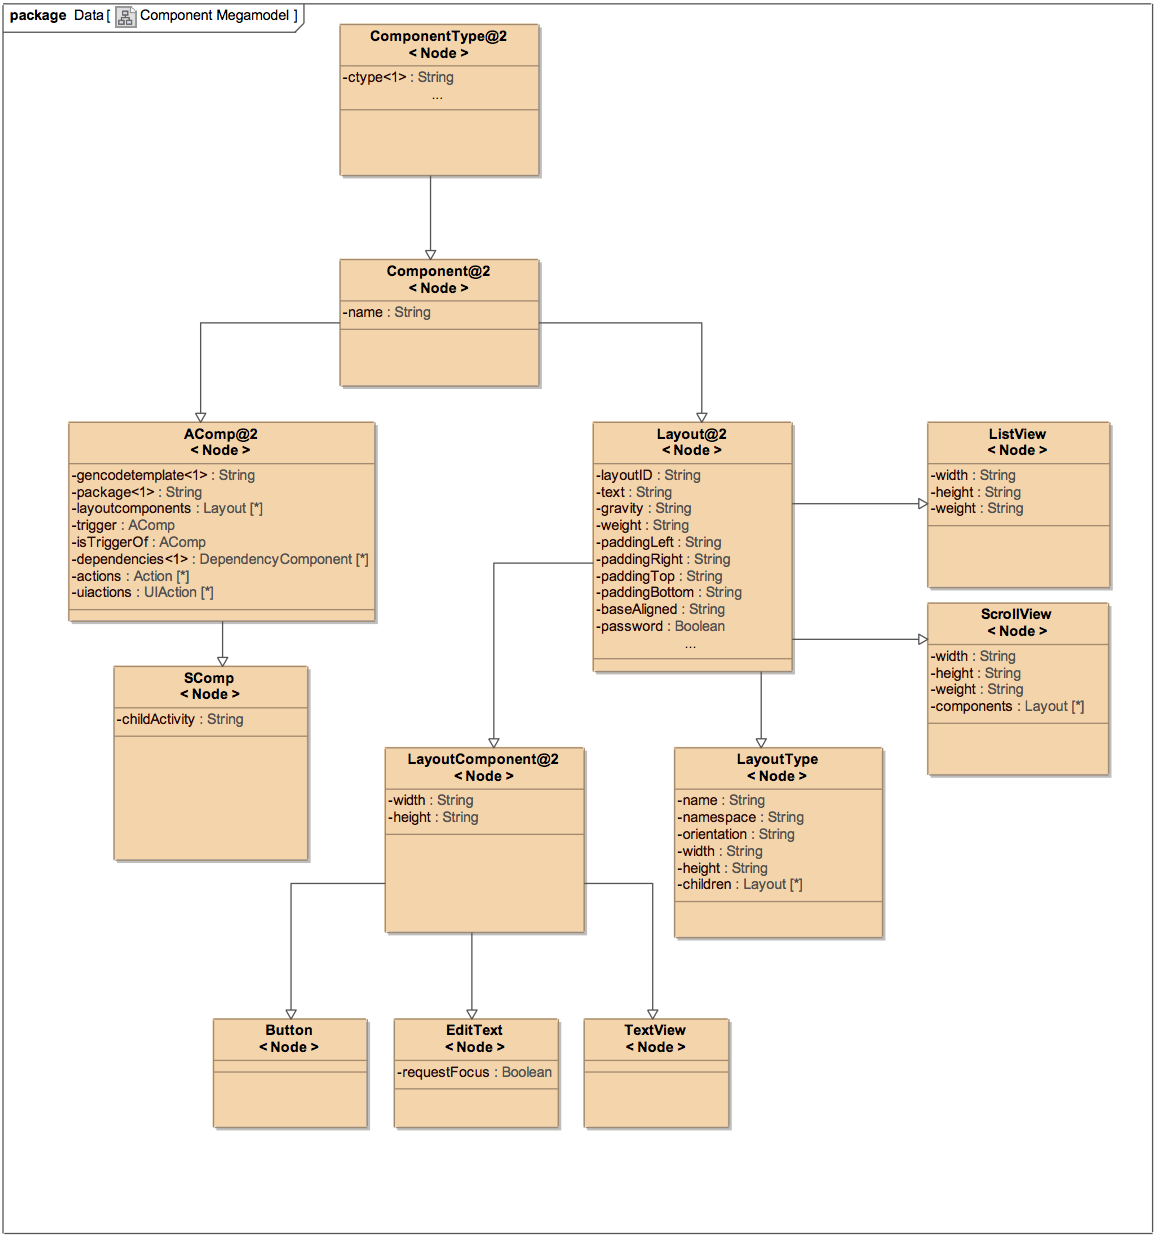
\includegraphics[width=1.0\textwidth]{images/chap6_component_megam.png}
\caption{Component Class Diagram}
\label{fig:component_megamodel}
\end{figure}

\subsection{Component}

The \texttt{Component} meta-model is listed in Listing ~\ref{component-mm}.

\begin{lstlisting}[label=component-mm,caption=Component meta-model, captionpos=t]
Model Component@2 {
	
	abstract Node ComponentType {
		ctype@1		: String{id};
	}

	Node Component : ComponentType {
		name			: String;
	}

	Node ComponentData@1 {
		name 		: String;
		value 		: String;
	}
	
	Node Layout : Component {
		layoutID		: String;
		text 			: String;
		gravity			: String;

		paddingLeft 	: String;
		paddingRight	: String;
		paddingTop 		: String;
		paddingBottom 	: String;
		baselineAligned : String;
	}

	// e.g. Button, EditText, TextView, ...
	Node LayoutComponent@2 : Layout {
		width			: String;
		height			: String;
		weight			: String;
	}

}
\end{lstlisting}
As we can see, this meta-model has a potency level of 2. This means that we have three levels in the meta-model. At the highest level, we define an abstract \texttt{Component} meta-model. Going down one level, we have defined the \texttt{AndroidComponent} itself (e.g. \textit{SMS}) and at level 0, we instantiate the component in our model. All components are of type \texttt{AndroidComponent} which is a subtype of \texttt{Component}. This component will be discussed in the next section. \texttt{LayoutComponent} is another component that inherits from our \texttt{Component} meta-model. It is used to describe the layout elements of an \texttt{Activity} and has a potency of two. It follows the same instantiation scheme as an \texttt{AndroidComponent} does.

\subsection{AndroidComponent}

\begin{lstlisting}[label=androidcomponent-mm,caption=AndroidComponent meta-model, captionpos=t]
load "Component"
load "AndroidAction"
load "UIAction"

Model AndroidComponent@2 imports Component, AndroidAction, UIAction {

	// Android component for semantics and extensibility
	Node AComp : Component {
		gencodetemplate@1 		: String;

		package@1 				: String;
		layoutcomponents@2 		: LayoutComponent@0[*];

		// Trigger can be another component (e.g. GeoComponent)
		trigger 				: AComp@0;

		// isTriggerOf defines the bi-directional connection with another component
		// a component could be the trigger of another component or a layoutcomponent
		isTriggerOf 			: AComp@0;
		dependencies@1 			: DependencyComponent[*];

		properties@1 			: ComponentData[*];
		
		// actions extend the action() method, so users can extend a component's functionality
		actions 				: Action[*];
		// uiactions are actions on a layoutcomponent
		uiactions 				: UIAction[*];
	}

	Edge Trigger@(2)(AComp.trigger, AComp.isTriggerOf) {
		actions 				: Action[*];
	}

	Node SComp : AComp {
		childActivity	: String;
	}
}
\end{lstlisting}
The \texttt{AndroidComponent} meta-model contains a \texttt{Node} that inherits from \texttt{Component}. \texttt{AComp} contains all necessary slots to instantiate and generate an Android component. At potency level one, we instantiate the EGL template to be used for generating the component code (in Java), the Java package that should be used, optional dependencies (regular Java classes) or properties to be associated with the component. An example of a possible property is a telephone number for sending an SMS. At the instantiation level, we can instantiate the remaining fields of \texttt{AComp}, such as \textit{layoutcomponents} or \textit{actions}. A \texttt{trigger} or \texttt{isTriggerOf} field can be specified, which enables local communication between two components. For example, when the trigger of a \texttt{GeoComponent} is fired, it passes its location to another component (e.g. \texttt{SMSComponent}), after which this component can use the location data to perform an action (e.g. send an SMS). This trigger can additionally be extended by using the \texttt{Trigger} edge. Through the \texttt{Trigger} edge, we can specify a list of actions to be executed when a trigger is fired. The trigger behavior is implicit to each component and cannot be changed. For instance, a \texttt{GeoComponent} will only trigger when a new location is found. \\ \\
Apart from a normal \texttt{AComp} node, a modeler can also instantiate components of type \texttt{SComp}. These components are used to represent client/server components. Typically, an instantiation of \texttt{SComp} communicates with a server. An example of this is the \texttt{DropboxComponent}. These type of components are usually embedded in an activity and could optionally have a child activity. For instance in a \texttt{DropboxComponent}, we usually want to show additional information on documents found in a Dropbox repository. This additional information will be shown through a child activity that is specified in a Dropbox instantiation of type \texttt{SComp}. \\

\subsection{Example Component}

As an example, we will show the Dropbox component, both on potency level one as well as on the instantiation level. The model for potency level one is listed in Listing ~\ref{dropbox-m}.

\begin{lstlisting}[label=dropbox-m,caption=Dropbox model, captionpos=t]
load "Component"

AndroidComponent dropboxComponent {
	
	SComp Dropbox {
		ctype = "dropbox";
		gencodetemplate = "dropbox.egl";

		folder 		: String;
		key 		: String;
		secret 		: String;
	}

}
\end{lstlisting}
At this level, we specify the template to generate the Java Dropbox component. We also introduce new slots that represent the name of the folder that should be used as a repository, together with the token key and token secret to authenticate with OAuth \cite{OAuth}. This level should and will never be visible to a developer. A modeler is only concerned about the instantiation level. The model instantiation is listed in Listing ~\ref{dropbox-inst}.

\begin{lstlisting}[label=dropbox-inst,caption=Dropbox instantiation, captionpos=t]
Dropbox dropbox {
	layoutcomponents = [dropboxButton, dirContentButton, contentText, dirContent];
	actions = [];
	uiactions = [triggerDropbox];

	childActivity = "DropboxItemActivity";
	folder = "/Thesis/";
	key = "KEY";
	secret = "SECRET";
}
\end{lstlisting}
We have defined a few layout components that make up the layout of the Dropbox activity. For instance, the \texttt{dirContentButton} value is used to grab the content of the Dropbox folder and the \texttt{dirContent} value represents the list that contains all filenames after the content is fetched from the Dropbox folder, that is specified by the folder, key and secret fields. When clicking on an item in a list, the activity that is specified in the \texttt{childActivity} field is initiated. This activity allows a user to make comments on a file (e.g. a research paper) in the specified Dropbox folder.

\section{Server}

In this section, we will review the \texttt{Server} meta-model and very briefly discuss the implementation details. The server component was written in Javascript and uses WebSockets for bi-directional communication, i.e. communication from client to server and vice versa.

\subsection{Meta-model}

The \texttt{Server} meta-model is quite straight-forward and the more complex parts are implemented in Node.js. \texttt{Server} is embedded into the \texttt{Application} meta-model. The code is listed in Listing ~\ref{server-mm}.

\begin{lstlisting}[label=server-mm,caption=Server meta-model, captionpos=t]
load "Session"
load "AndroidComponent"

Model Server imports Session, AndroidComponent {

	Node Server {
		name 			: String;
		session 		: SessionObject;
		host 			: String;
		port 			: String;
		components 		: Component@0[*];
	}
}
\end{lstlisting}
The host and port for the server can be set, together with the components that should be included in the server. Apart from that, a modeler should also set a \texttt{SessionObject} node. This node simply contains a list of users that are able to authenticate to the server, together with their role. 

\subsection{Javascript and WebSockets}

The most relevant part of the \texttt{Server} meta-model lies in the implementation in Javascript. In order to realize both asynchronous as well as synchronous communication, Node.js \cite{NodeJS} was used together with WebSockets:
\begin{quotation}
The WebSocket specification - developed as part of the HTML5 initiative - introduced the WebSocket JavaScript interface, which defines a full-duplex single socket connection over which messages can be sent between client and server. The WebSocket standard simplifies much of the complexity around bi-directional web communication and connection management \cite{WebSockets}. 
\end{quotation}
If we send all our data packets through a \texttt{WebSocket}, we can communicate with our server in \textit{near real-time}, because there is bi-directional communication between the client and server. Combining this with a server implementation in Node.js, we leverage Javascript to implement a data-intensive real-time application suited for multiple devices:
\begin{quotation}
Node.js is a platform built on Chrome's JavaScript runtime for easily building fast, scalable network applications. Node.js uses an event-driven, non-blocking I/O model that makes it lightweight and efficient, perfect for data-intensive real-time applications that run across distributed devices.
\end{quotation}
Since all communication works through WebSockets, the server implementation is decoupled from any Android application a developer may model. If at some point the modeling framework has to be adapted to generate iOS applications, nothing has to be changed to the Javascript server implementation. The only requirement is a \texttt{WebSocket} library on the client side (iOS/Android/web).

\section{Code Generation}

In this section, we will explain the code generation details of Metadepth and the collaborative modeling framework. First, we will briefly explain the Epsilon Generation Language (EGL) syntax. Afterwards, we will show an example of the code generation of the activities in an Android application.

\subsection{Epsilon Generation Language}

EGL is a template-based model-to-text language for generating code, documentation and other textual artefacts from models. EGL supports content-destination decoupling, protected regions for mixing generated with hand-written code, and template coordination \cite{EpsilonGenerationLanguage}. \\ \\
The concrete syntax of EGL closely resembles the style of other template-based code generation languages, such as PHP \cite{EpsilonBook}. Any text enclosed in a tag pair \textit{[\%} \textit{\%]} is used to delimit a dynamic code section. Text not inclosed in a tag pair is considered static code. Listing ~\ref{egl-template} illustrates the use of dynamic and static code sections to from a basic EGL template. 
\begin{lstlisting}[label=egl-template,caption=EGL template, captionpos=t]
?[% for (i in Sequence{1..5}) { %]
	i is [%= i %]
[% } %]
\end{lstlisting}
The structure of this basic template is used for the generation of Java code in the collaborative modeling framework. The next subsection shows an example of a real EGL template used in the collaborative modeling framework.

\subsection{Example}

Finally, after a model has been created, a developer can initiate the code generation phase. This phase loads a set of EGL files and traverses each model that has been created. A typical code generation process is implemented as follows:

\begin{lstlisting}[label=codegen-app,caption=Android code-generation, captionpos=t]
// generate main Android app
var t : Template := TemplateFactory.load(basePath+'genActivity.egl');
if (application.activities.isDefined() and application.activities.size() > 0) {
	for (activity in application.activities) {
		if (activity.main == true) {
			"populating server var".println();
			if (application.server.isDefined()) {
				t.populate('server', application.server);
			}
		}
		t.populate('activity', activity);
		t.populate('application', application);
		t.populate('path', path);
		t.populate('basePath',    basePath);
		t.populate('compPath',    compPath);
		t.populate('codePath',	  codePath);
		t.process();
		t.generate(codePath + 'src/' + path + activity.name + '.java');
	
		var l : Template := TemplateFactory.load(basePath+'genDependency.egl');
		if (activity.content.isDefined() and activity.content.size() > 0) {
			for (c in activity.content) {
				if (c.dependencies.isDefined() and c.dependencies.size() > 0) {
					for (d in c.dependencies) {
						l.populate('dependency', d);
						l.populate('basePath',    basePath);
						l.populate('compPath',    compPath);
						l.process();
						l.generate(codePath + 'src/' + path + d.name + '.java');
					}
				}
			}
		}
	}
}
\end{lstlisting}
This listing iterates all defined activities and generates the Java \texttt{Activity} files. Lines 11 through 16 populate the template with variables we need to generate the target (Java) code. The \texttt{populate} method passes variables in the source formalism and map these onto a name. For example, in line 11, we assigned the activity variable to 'activity' in the EGL template that will be called. Line 17 processes all this information and line 18 finally calls the template we initiated in line 2. The template is initiated by calling the \texttt{generate} method. This method expects one parameter, the location on the file system of the file that is to be generated.
